\documentclass[8pt, serif, xcolor=table]{beamer}

\usepackage{textpos}
\usepackage{paralist}
\usepackage{enumitem}
\usepackage{expdlist}
\usepackage{subfigure}
\usepackage{amssymb, amsmath, amsthm}
\everymath{\displaystyle}

\usepackage[T1]{fontenc}
\usepackage{mathpazo}

\definecolor{shade}{RGB}{240,240,240}

\newcommand{\mono}[1]{\texttt{#1}}
\newcommand{\textt}[1]{\ensuremath{\text{\mono{#1}}}}
\newcommand{\mathmono}[1]{\ensuremath{\text{\mono{#1}}}}
\newcommand{\nonterm}[1]{\ensuremath{\text{\mono{<#1>}}}}
\newcommand{\term}[1]{\ensuremath{\text{\mono{`#1'}}}}
\newcommand{\any}[0]{\ensuremath{\left\langle\bigtriangleup\right\rangle}}
\newcommand{\D}{$\Delta$}

\newcommand{\makeTable}[6][htbp!]
{
	\begin{table}[#1]
	\centering
	\begin{tabular}{#4}
	#5\\
	#6\\
	\end{tabular}
	\end{table}
}

\newcommand{\includeFigure}[4][htbp!]
{
	\begin{figure}[#4]
	\centering
	\IfDecimal{#1}
	{
		\includegraphics[scale=#1]{figures/#2}
	}
	{
		\includegraphics[#1]{figures/#2}
	}
	\caption[]{#3}
	\label{figure:#2}
	\end{figure}
}

\usepackage{clrscode3e}
\usepackage{verbatim}
\usepackage{listings}
\lstset
{
	tabsize=2,
	numbers=left,
	breaklines=true,
	foregroundcolor=\color{shade},
	framexleftmargin=0.05in,
	basicstyle=\ttfamily\small,
	numberstyle=\tiny,
%  keywordstyle=\color{green},
%	stringstyle=\color{red},
%	commentstyle=\color{ForestGreen},
  keywords={input},
  mathescape=true,
  captionpos=b,
  escapeinside={(*@}{@*)},
  language=haskell
}



\setbeamercolor{title}{fg=shade}
\setbeamercolor{frametitle}{fg=shade}
\setbeamercolor{normal text}{fg=shade}
\setbeamercolor{background canvas}{bg=black}
\setbeamercolor{bibliography item}{fg=shade}
\setbeamercolor{bibliography entry author}{fg=shade}
\setbeamertemplate{bibliography item}[text]

\newcommand{\bi}{$\bullet$\ }

\title{Termination analysis of first order programs}
\author{Oleksandr Shturmov}

\begin{document}

\begin{frame}

\titlepage

\end{frame}

% Use danish to have a more natural discussion. This may require us to change
% along the way as the concepts become too entangled in english terms.

\begin{frame}

\frametitle{Overview}

\tableofcontents

\end{frame}

\begin{frame}[plain]

$$H(M,x)=\left\{
\begin{array}{ll}
true&M\ \text{halts on}\ x,\\
false&M\ \text{does not halt on}\ x.
\end{array}
\right.$$

\end{frame}

\begin{frame}

$$H(M,x)=\left\{
\begin{array}{ll}
true&M\ \text{halts on}\ x,\\
false&M\ \text{does not halt on}\ x.
\end{array}
\right.$$

$$F(M)=\left\{
\begin{array}{ll}
true& H(M,M) \leadsto false,\\
false& H(M,M) \leadsto true.
\end{array}
\right.$$

$$\text{Consider}\ F(F).$$

\end{frame}

\begin{frame}

$$H(M,x)=\left\{
\begin{array}{ll}
true&M\ \text{halts on}\ x,\\
false&M\ \text{does not halt on}\ x,\\
unknown&M\ \text{may or may not halt on}\ x.
\end{array}
\right.$$

% The definition used in the report.

\end{frame}

\begin{frame}

$$H(M,x)=\left\{
\begin{array}{ll}
true&M\ \text{halts on}\ x,\\
unknown&M\ \text{may or may not halt on}\ x.
\end{array}
\right.$$

% To be honest, given the size-change termination principle, this definition is
% even better.

\end{frame}

\begin{frame}

\begin{center}

``Unfortunately, many have drawn too strong of a conclusion about the prospects
of automatic program termination proving and falsely believe we are always
unable to prove termination, rather than the more benign consequence that we
are unable to always prove termination.''

\end{center}

\begin{flushright}
\cite{cook2011}
\end{flushright}

\end{frame}

\begin{frame}

%\frametitle{The size-change termination principle}

\begin{center}

``The {\bf size-change termination principle} for a first-order functional
language with well-founded data is: a program terminates on all inputs if
\emph{every infinite call sequence} (following program control flow) would
cause an infinite descent in some data values.''

\end{center}

\begin{flushright}
\cite{size-change}
\end{flushright}

\end{frame}

\begin{frame}

\begin{center}

{\fontsize{40}{20} $\Delta$}

\vspace{0.5in}

An untyped, call-by-value, functional first-order language.

\end{center}

\end{frame}

\section{Data}

\D{} is a simple language where the emphasis is on the sizes of data. Hence,
the way that data values are constructed does not have to be particularly
practical, but all values have to be well founded and easily comparable.

The language \D{} is untyped, and represents all data in terms of
\emph{unlabeled ordered binary trees}, henceforth referred to as simply,
\emph{binary trees}. Such a tree is recursively defined as follows:

\begin{definition}

A binary tree is a set that is either empty, heneceforth refferred to as leaf,
or contains a single unlabeled node with two binary trees as it's left and
right child, henceforth simply reffered to as node. We'll refer to the set of
all possible values in \D{} as $\mathbb{B}$.

\end{definition}

To operate on such trees we'll require a few primitives, namely a
representation of leafs, recursive construction and destruction of nodes, as
well as a way to tell nodes and leafs apart. Most of these will be derived in
the operational semantics of \D{}\footnote{See \referToSection{d-sos}.},
however, we do require the following basic definitions:

\begin{definition}

Let the atom $0$ represent a leaf binary tree.

\end{definition}

\begin{definition}

The function $\cdot
:\mathbb{B}\times\mathbb{B}\rightarrow\mathbb{B}$ constructs a node with the
two arguments as it's left and right child, respectively. 

\end{definition}


\section{Syntax}\label{section:d-syntax}

We describe the syntax of \D in terms of an extended Backus-Naur
form\footnote{The extension lends some constructs from regular expressions to
achieve a more concise dialect. The extension is described in detail in
\referToAppendix{ebnf}.}. This is a core syntax definition, and other, more
practical, syntactical features may be defined later on as needed.

\begin{align}
\nonterm{expression}\ ::=&\ \nonterm{value}\ (\ \term{.}\ \nonterm{expression}
\ )\ ?\\
\nonterm{value}\ ::=&\ \term{0}\ |\ \term{(}\ \nonterm{value}\ \term{)}\ |
\ \nonterm{application}\\
\nonterm{application}\ ::=&\ \nonterm{name}
\ \nonterm{expression}^*\\
\nonterm{function}\ ::=&\ \nonterm{name}\ \nonterm{pattern}^*
\ \term{:=}\ \nonterm{expression}\\
\nonterm{pattern}\ ::=&\ \nonterm{pattern-value}\ (\ \term{.}
\ \nonterm{pattern}\ )\ ?\\
\nonterm{pattern-value}\ ::=&\ \term{0}\ |\ \term{\_}\ |\ \term{(}
\ \nonterm{pattern}\ \term{)}\ |\ \nonterm{name}\\
\nonterm{name}\ ::=&\ [\term{a}\mathmono{-}\term{z}]
\ \left (\ [\term{-}\ \term{a}\mathmono{-}\term{z}]^*
\ [\term{a}\mathmono{-}\term{z}]\ \right )?
\end{align}

The term $\term{\_}$ in $\nonterm{pattern-value}$ is the conventional wildcard
operator; it indicates a value that won't used by the function declaration, but
allows us to keep the same function signature. We define the \emph{signature}
of a function as follows:

\begin{definition}

A function signature in D consists of the function name and the number of
parameters it has.

\end{definition}

% TODO this should be clear from the semantics.

% Multiple wildcards in the parameter list indicate possibly different value
% arguments, while multiple occurances of the same variable name in the parameter
% list are disallowed.

\begin{frame}

\begin{textblock}{1}(13.8,-3.8)$(15)$\end{textblock}

%\frametitle{Symbols}

\makeTable[h!]
{sos-definitions}
{}
{lccc}
{\textbf{Description}&\textbf{Instance}&\textbf{Finite list}&\textbf{Space}}
{
&&&\\
Expression & $x$ & $X$ & $\mathbb{X}$\\
Element (of an expression) & $e$ & $E$ & $\mathbb{E}$\\
Function & $f$ & $F$ & $\mathbb{F}$\\
Clause & $c$ & $C$ & $\mathbb{C}$\\
Pattern & $p$ & $P$ & $\mathbb{P}$\\
Value (think ``binary'') & $b$ & $B$ & $\mathbb{B}$\\
Name (think ``variable'') & $v$ & $V$ & $\mathbb{V}$\\
Program ($p$ was taken) & $r$ & $R$ & $\mathbb{R}$\\
Shape & $s$ & $S$ & $\mathbb{S}$
}

\end{frame}

\begin{frame}

\begin{textblock}{1}(13.8,-3.5)$(14)$\end{textblock}

\frametitle{\D{}, syntax}

\setcounter{equation}{0}

\begin{align*}
\nonterm{program}\ \textt{::=}&\ \nonterm{clause}^{\color{red}\textt{\bf +}}
\ \nonterm{expression}
& \\
\nonterm{expression}\ \textt{::=}&\ \nonterm{element}\ \textt{(}\ \term{.}
\ \nonterm{expression}\ \textt{)}\ \textt{?}
& x\\
\nonterm{element}\ \textt{::=}&\ \term{0}\ \textt{|}\ \term{(}
\ \nonterm{element}\ \term{)}\ \textt{|}\ \nonterm{name}\ \textt{|}
\ \nonterm{application}
& e\\
\nonterm{application}\ \textt{::=}&\ \nonterm{name}
\ \nonterm{expression}^{\color{yellow}\textt{*}}
& \left\langle v,X \right\rangle \\
\nonterm{clause}\ \textt{::=}&\ \nonterm{name}
\ \nonterm{pattern}^{\color{yellow}\textt{*}}\ \term{:=}
\ \nonterm{expression}{\color{green}\term{;}}
& c=\left\langle v, P, x \right\rangle \\
\nonterm{pattern}\ \textt{::=}&\ \nonterm{pattern-element}\ \textt{(}
\ \term{.}\ \nonterm{pattern}\ \textt{)}\ \textt{?}
& p\\
\nonterm{pattern-element}\ \textt{::=}&\ \term{0}\ \textt{|}\ \term{\_}
\ \textt{|}\ \term{(}\ \nonterm{pattern}\ \term{)}\ \textt{|}\ \nonterm{name}
& p\\
\nonterm{name}\ \textt{::=}&\ \textt{[}\term{a}\mathmono{-}\term{z}\textt{]}
\ \textt{(}\ \textt{[}\term{-}\ \term{a}\mathmono{-}\term{z}\textt{]}^\textt{*}
\ \textt{[}\term{a}\mathmono{-}\term{z}\textt{]}\ \textt{)}\ \textt{?}
& v
\end{align*}

% e in this case could've well been x.. %

\end{frame}

\begin{frame}

\begin{textblock}{1}(13.8,-3.5)$(14)$\end{textblock}

\frametitle{\D{}, syntax}

\setcounter{equation}{0}

\begin{align*}
\nonterm{program}\ \textt{::=}&\ \nonterm{clause}^{\color{red}\textt{\bf +}}
\ \nonterm{expression}
& \\
\nonterm{expression}\ \textt{::=}&\ \nonterm{element}\ \textt{(}\ \term{.}
\ \nonterm{expression}\ \textt{)}\ \textt{?}
& x\\
\nonterm{element}\ \textt{::=}&\ \term{0}\ \textt{|}\ \term{(}
\ \nonterm{element}\ \term{)}\ \textt{|}\ \nonterm{name}\ \textt{|}
\ \nonterm{application}
& e\\
\nonterm{application}\ \textt{::=}&\ \nonterm{name}
\ \nonterm{expression}^{\color{yellow}\textt{*}}
& \left\langle v,x \right\rangle \\
\nonterm{clause}\ \textt{::=}&\ \nonterm{name}
\ \nonterm{pattern}^{\color{yellow}\textt{*}}\ \term{:=}
\ \nonterm{expression}{\color{green}\term{;}}
& c=\left\langle v, p, x \right\rangle \\
\nonterm{pattern}\ \textt{::=}&\ \nonterm{pattern-element}\ \textt{(}
\ \term{.}\ \nonterm{pattern}\ \textt{)}\ \textt{?}
& p\\
\nonterm{pattern-element}\ \textt{::=}&\ \term{0}\ \textt{|}\ \term{\_}
\ \textt{|}\ \term{(}\ \nonterm{pattern}\ \term{)}\ \textt{|}\ \nonterm{name}
& p\\
\nonterm{name}\ \textt{::=}&\ \textt{[}\term{a}\mathmono{-}\term{z}\textt{]}
\ \textt{(}\ \textt{[}\term{-}\ \term{a}\mathmono{-}\term{z}\textt{]}^\textt{*}
\ \textt{[}\term{a}\mathmono{-}\term{z}\textt{]}\ \textt{)}\ \textt{?}
& v
\end{align*}

% e in this case could've well been x.. %

\end{frame}

\begin{frame}

\begin{textblock}{1}(13,-3.5)$(15,36)$\end{textblock}

\frametitle{Functions in \D{}}

$$f = \left\langle v, C \right\rangle \quad \text{s.t.} \quad \forall\
\left\langle v',\_,\_ \right\rangle \in C\ \left( v'=v \right)$$

%\vspace{1in}

\begin{center}

Pattern matching is ensured {\bf exhaustive} at compile time, i.e.

$$\forall\ b \in \mathbb{B}\ \exists\ c \in C\ c\succ b.$$

WLOG, $c = \left\langle p,x \right\rangle$.

\end{center}

\end{frame}

\begin{frame}[fragile]

\begin{textblock}{1}(13.8,-3.5)$(15)$\end{textblock}

\frametitle{Patterns and shapes}

\begin{columns}
\column{0.5\textwidth}
\begin{center}
\mono{f (\_.0).0 := ...}
\end{center}

\column{0.5\textwidth}
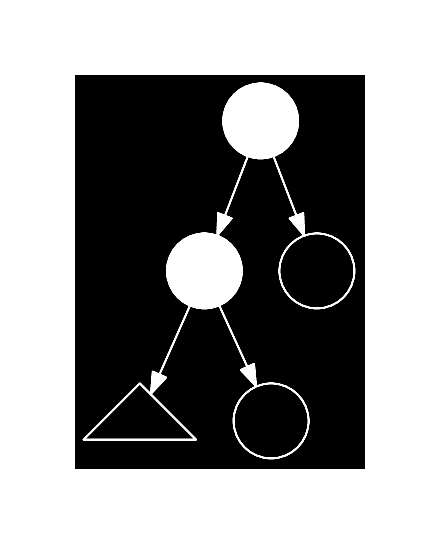
\includegraphics[scale=0.5]{figures/shape}

\end{columns}

\end{frame}

\begin{frame}[fragile]

\begin{codebox}
\Procname{$\proc{Ensure-Exhaustive}(c : C)$}
\li $P_{siblings} \gets \proc{Get-Siblings}(c)$
\li $C' \gets [c]$
\li \For $c'\in C$ \Do
\li $(P_{success},P_{fail}) \gets \proc{Match-Clause-To-Siblings}(c,P_s)$
\li \For $p\in P_{success}$ \Do
\li $c'' \gets \proc{Clone}(c')$
\li $\proc{Merge-Pattern}(c'',p)^{\color{green}\textt{\bf *}}$
\li $C' \gets c' : C'$ \End
\li $P_{siblings} \gets P_{fail}$ \End
\li \Return $C'$
\end{codebox}

{\bf Invariants:}

\begin{itemize}

\item \bi $P_{siblings}$ is always a list of siblings that wasn't matched by
any forthcoming clause.

\item \bi $P_{success}$ and $P_{fail}$ are always sibling lists.

\end{itemize}

\end{frame}

\begin{frame}

\begin{center}

\Huge Demo

\end{center}

\end{frame}



\begin{frame}

\frametitle{Programs in \D{}}

$$r=\left\langle F, x \right\rangle$$

\end{frame}

\begin{frame}

\frametitle{Observed mistakes}

\begin{itemize}

\item List indexing

\begin{itemize}

\item \bi Lists are sometimes 0-indexed rather than 1-indexed.

\item \bi $\forall\ \{i\mid 0\geq i < |P|\}$ should obviously be $\forall\
\{i\mid 0< i \leq |P|\}$.

\end{itemize}

\item $\Cup$

\item Superflous conditions.

\end{itemize}

\end{frame}

\begin{frame}

\section{References}

\frametitle{References}

\begin{thebibliography}{2}

\bibitem[Cook et al., 2011]{cook2011} B. Cook, A. Podelski \& A.  Rybalchenko,
\emph{Proving program termination}, Communications ACM Vol. 54(5), 2011, 88--98.

\bibitem[Lee et al., 2001]{size-change} Chin Soon Lee, Neil D. Jones, and Amir
M. Ben-Amram. 2001. \emph{The size-change principle for program termination},
In Proceedings of the 28th ACM SIGPLAN-SIGACT symposium on Principles of
programming languages (POPL '01), ACM, New York, NY, USA, 81--92.

\end{thebibliography}

\end{frame}


\end{document}
